\documentclass[border=6pt]{standalone}
\usepackage{tikz}
\usepackage{amsmath,amssymb}
\usepackage{helvet}\renewcommand{\familydefault}{\sfdefault}
\usetikzlibrary{positioning,arrows.meta,backgrounds,fit,shapes.geometric,calc,decorations.pathreplacing}

\definecolor{frblue}{HTML}{1f78b4}
\definecolor{frlight}{HTML}{a6cee3}
\definecolor{frgreen}{HTML}{33a02c}
\definecolor{frgrey}{HTML}{949494}
\definecolor{frorange}{HTML}{ff7f00}

\begin{document}
\begin{tikzpicture}[
  font=\footnotesize,
  >={Latex[length=1.8mm]},
  data/.style={draw=frgrey!55,rounded corners=2pt,fill=frgrey!10,align=center,inner sep=3pt,minimum height=6mm,text width=3.5cm},
  stem/.style={draw=frblue!55,rounded corners=2pt,fill=frblue!12,align=center,inner sep=3pt,minimum height=6mm,text width=3.6cm},
  ln/.style={draw=frblue!40,rounded corners=1.5pt,fill=frblue!5,align=center,font=\scriptsize,inner sep=2pt,minimum height=3.6mm,text width=3.2cm},
  ssmb/.style={draw=frblue!60,rounded corners=2pt,fill=frlight!60,align=center,inner sep=2.5pt,minimum height=6.5mm,text width=3.2cm},
  ffnb/.style={draw=frblue!55,rounded corners=2pt,fill=frlight!25,align=center,inner sep=2.5pt,minimum height=5mm,text width=3.2cm},
  dec/.style={draw=frblue!55,rounded corners=2pt,fill=frblue!16,align=center,inner sep=3pt,minimum height=6mm,text width=3.6cm},
  circ/.style={draw=frblue!60,circle,inner sep=0pt,minimum size=3.2mm,font=\scriptsize},
  cond/.style={draw=frorange!70,rounded corners=2pt,fill=frorange!12,align=center,inner sep=2.5pt,font=\scriptsize,text width=1.9cm},
  head/.style={draw=frgreen!60,rounded corners=2pt,fill=frgreen!14,align=center,inner sep=3pt,minimum height=6mm,text width=2.7cm},
  aux/.style={draw=frgrey!55,rounded corners=2pt,fill=frgrey!8,align=center,font=\scriptsize,inner sep=2.5pt,text width=2.5cm},
  flow/.style={->,frblue!75,semithick},
  res/.style={->,frgrey!60,semithick,rounded corners=2pt},
  side/.style={font=\scriptsize,text=frgrey!80},
  stgcap/.style={font=\small\bfseries,text=frblue!85},
]

% ============================================================= STAGE A : DATA
\def\ax{0}
\node[data] (src) at (\ax,0) {\textbf{any genotypes}\\[1pt]{\scriptsize phased \emph{or} unphased $\cdot$ polarized \emph{or} unpolarized}};
\node[data,above=5mm of src] (gm) {genotype matrix + SNP positions\\{\scriptsize filter to biallelic, segregating}};
\node[data,above=5mm of gm,fill=frgrey!14] (feat) {composite-LD featurizer\\{\scriptsize \texttt{GTTokenFeaturizer} — Rogers–Huff dosages}};
\draw[flow] (src) -- (gm);
\draw[flow] (gm) -- (feat);
% token strip
\node[above=7mm of feat] (tc) {};
\foreach \i/\x in {1/-1.5,2/-0.75,3/0,4/0.75,5/1.5}{
  \node[draw=frblue!45,fill=frblue!8,minimum width=4.5mm,minimum height=6.5mm,inner sep=0]
    (tok\i) at ($(tc)+(\x,0)$) {};}
\node[side,above=0.4mm of tok3,align=center] {tokens $x_1\!\dots x_L$: one per SNP\\ features: $r^2_{5/25/50\,\text{kb}}$, two-locus configs, MAF, $\pi$, spacing};
\draw[flow] (feat) -- (tok3.south);

% ============================================================= STAGE B : MODEL
\def\bx{5.9}
\node[stem] (stem) at (\bx,0) {\texttt{SNP-token stem}\\{\scriptsize embed + depthwise conv $k{=}3,7,15 \to d{=}256$}};
\node[circ,above=4mm of stem] (pe) {$+$};
\node[side,left=1mm of pe,align=right,text width=1.7cm] {learned\\positional emb.};
\draw[flow] (stem) -- (pe);
% --- one BiMambaBlock (pre-norm, two residual sublayers) ---
\node[ln,above=5.5mm of pe]  (ln1) {LayerNorm};
\node[ssmb,above=2mm of ln1] (ssm) {bidirectional Mamba-2\\{\scriptsize forward $\rightleftarrows$ backward scan}};
\node[circ,above=2.5mm of ssm] (a1) {$+$};
\node[ln,above=2.5mm of a1] (ln2) {LayerNorm};
\node[ffnb,above=2mm of ln2] (ffn) {feed-forward $256\!\to\!1024\!\to\!256$};
\node[circ,above=2.5mm of ffn] (a2) {$+$};
\draw[flow] (pe) -- (ln1);
\draw[flow] (ln1) -- (ssm);
\draw[flow] (ssm) -- (a1);
\draw[flow] (a1) -- (ln2);
\draw[flow] (ln2) -- (ffn);
\draw[flow] (ffn) -- (a2);
% residual skips (right side)
\draw[res] (pe.east) -- ++(1.75,0) |- (a1.east);
\draw[res] (a1.east) -- ++(1.75,0) |- (a2.east);
% block background + label
\begin{scope}[on background layer]
  \node[draw=frblue!35,dashed,rounded corners=3pt,fill=frblue!3,
        fit=(ln1)(a2),inner sep=3pt] (blk) {};
\end{scope}
\node[side,text=frblue!80,above left=0mm and -1mm of blk.north west,anchor=south west] {\texttt{BiMambaBlock}};
% encoder brace
\draw[decorate,decoration={brace,amplitude=5pt},frblue!70]
  ($(blk.south west)+(-0.15,0)$) -- ($(blk.north west)+(-0.15,0)$)
  node[midway,left=5pt,text=frblue!85,font=\scriptsize,align=center]{$\times6$ enc.\\ $\times4$ dec.\\ U-Net\\ skips};
% FiLM conditioning
\node[cond,left=4mm of ssm] (condn) {\textbf{FiLM} cond\\ $\log\mu,\ \log n_{\text{hap}}$\\ is\_gt, is\_folded};
\draw[->,frorange!85,semithick] (condn.east) -- (ssm.west);
% ============================================================= STAGE C : HEADS + MAP
\def\cx{12.0}
\coordinate (cxc) at (\cx,0);
\node[head] (bnll) at (cxc |- a2) {$\beta$-NLL head\\{\scriptsize \texttt{UncertaintyHead}}};
\draw[flow] (a2.north) -- ++(0,0.35) -| (bnll.north);
\node[align=center,below=5mm of bnll,font=\scriptsize] (mv)
  {mean $\hat\mu(x)$ \qquad var $\hat\sigma^2(x)$};
\draw[flow] (bnll) -- (mv);
% conversion
\node[align=center,below=3.5mm of mv,font=\scriptsize,text=frblue!90] (conv)
  {$\hat r(x)=e^{\hat\mu(x)}/(4N_e)$\\[2pt]
   $95\%\ \text{CI}=e^{\hat\mu\pm1.96\hat\sigma}/(4N_e)$};
\draw[flow] (mv) -- (conv);
% inferred map: a REAL minimal fastrho inference (a deCODE region, rate + 95% band)
\node[anchor=north,inner sep=1pt] (map) at (\cx,2.55) {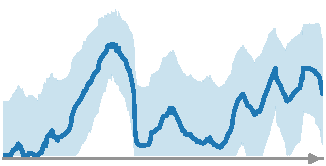
\includegraphics[width=3.7cm]{fig1_inset_map.pdf}};
\node[side,text=frblue!90,align=center,below=1.2mm of map]
  {per-SNP-interval rate $\pm\,95\%$ CI\\{\scriptsize (real deCODE inference)}};
\draw[flow] (conv) -- (map.north);

% ============================================================= TOP BANNER
\node[draw=frgrey!45,rounded corners=3pt,fill=frgrey!6,inner sep=5pt,
      text width=16.4cm,align=center,font=\scriptsize] (train) at (5.7,6.75)
  {\textbf{Trained once (amortized).}\;
   \texttt{msprime}\,+\,\texttt{stdpopsim} prior — demographies (constant / bottleneck / sawtooth / island) $\times$ sample sizes $\times$ hotspot maps
   $\;\to\;$ domain-randomized corpus $\;\to\;$
   \textcolor{frblue!90}{\textbf{one frozen model}}, applied to any dataset with no lookup table, no per-dataset tuning, no retraining};

% ============================================================= STAGE CAPTIONS
\node[stgcap] at (\ax,-1.35) {a\ \ \normalfont\footnotesize any genotypes $\to$ tokens};
\node[stgcap] at (\bx,-1.35) {b\ \ \normalfont\footnotesize amortized bidirectional SSM (Mamba-2)};
\node[stgcap] at (\cx,-1.35) {c\ \ \normalfont\footnotesize calibrated map in one forward pass};

% ============================================================= INTER-STAGE FLOW
% drawn on the background layer so it passes BEHIND the FiLM box, not across it
\begin{scope}[on background layer]
  \draw[->,frblue!45,line width=1.6pt] (tok5.east) to[out=0,in=150] ($(stem.north west)+(0.1,0.05)$);
\end{scope}

\end{tikzpicture}
\end{document}
